\documentclass[11pt,]{article}
\usepackage{mathpazo,mathabx}
\usepackage{amssymb,amsmath}
\usepackage{ifxetex,ifluatex}
\usepackage{fixltx2e} % provides \textsubscript
\ifnum 0\ifxetex 1\fi\ifluatex 1\fi=0 % if pdftex
  \usepackage[T1]{fontenc}
  \usepackage[utf8]{inputenc}
\else % if luatex or xelatex
  \ifxetex
    \usepackage{mathspec}
    \usepackage{xltxtra,xunicode}
  \else
    \usepackage{fontspec}
  \fi
  \defaultfontfeatures{Mapping=tex-text,Scale=MatchLowercase}
  \newcommand{\euro}{€}
    \setmainfont{Palatino}
    \setmonofont[Mapping=tex-ansi]{Inconsolata}
\fi
% use upquote if available, for straight quotes in verbatim environments
\IfFileExists{upquote.sty}{\usepackage{upquote}}{}
% use microtype if available
\IfFileExists{microtype.sty}{%
\usepackage{microtype}
\UseMicrotypeSet[protrusion]{basicmath} % disable protrusion for tt fonts
}{}
\usepackage[margin=1.5cm]{geometry}
\usepackage{longtable,booktabs}
\usepackage{graphicx}
\makeatletter
\def\maxwidth{\ifdim\Gin@nat@width>\linewidth\linewidth\else\Gin@nat@width\fi}
\def\maxheight{\ifdim\Gin@nat@height>\textheight\textheight\else\Gin@nat@height\fi}
\makeatother
% Scale images if necessary, so that they will not overflow the page
% margins by default, and it is still possible to overwrite the defaults
% using explicit options in \includegraphics[width, height, ...]{}
\setkeys{Gin}{width=\maxwidth,height=\maxheight,keepaspectratio}
\ifxetex
  \usepackage[setpagesize=false, % page size defined by xetex
              unicode=false, % unicode breaks when used with xetex
              xetex]{hyperref}
\else
  \usepackage[unicode=true]{hyperref}
\fi
\hypersetup{breaklinks=true,
            bookmarks=true,
            pdfauthor={},
            pdftitle={Copy-Paste Tracking: Fixing Spreadsheets Without Breaking Them},
            colorlinks=true,
            citecolor=blue,
            urlcolor=blue,
            linkcolor=magenta,
            pdfborder={0 0 0}}
\urlstyle{same}  % don't use monospace font for urls
\setlength{\parindent}{0pt}
\setlength{\parskip}{6pt plus 2pt minus 1pt}
\setlength{\emergencystretch}{3em}  % prevent overfull lines
\setcounter{secnumdepth}{0}

\title{Copy-Paste Tracking: Fixing Spreadsheets Without Breaking Them}
\author{true \and true}
\date{}

\begin{document}
\maketitle
\begin{abstract}
Spreadsheets are the most popular live programming environments, but
they are also notoriously fault-prone. One reason for this is that users
actively rely on copy-paste to make up for the lack of abstraction
mechanisms. Adding abstraction however, introduces indirection and thus
cognitive distance. In this paper we propose an alternative: copy-paste
tracking. Tracking copies that spreadsheet users make, allows them to
directly edit copy-pasted formulas, but instead of changing only a
single instance, the changes will be propagated to all formulas copied
from the same source. As a result, spreadsheet users will enjoy the
benefits of abstraction without its drawbacks.
\end{abstract}

\section{Introduction}\label{introduction}

Spreadsheet systems can easily be considered the most successful form of
programming. Winston {[}@Wins2001{]} estimates that 90\% of all analysts
in industry perform calculations in spreadsheets. Spreadsheet users
perform a range of diverse tasks with spreadsheets, from inventory
administration to educational applications and from scientific modeling
to financial systems. The financial business is a domain where
spreadsheets are especially prevailing. Panko {[}@Pank2006{]} estimates
that 95\% of U.S. firms, and 80\% in Europe, use spreadsheets in some
form for financial reporting.

Researchers have argued that the \emph{liveness} characteristics of
spreadsheets have contributed to the widespread success of spreadsheets
{[}@thesisFelienne{]} and we know from interviews with users that
liveness is important to them. They often start building a spreadsheet
with the end goal in mind, and manipulate the formulas until they obtain
the result they want.

The liveness characteristics of spreadsheets can be divided in two
categories:

\begin{itemize}
\item
  Direct manipulation: instead of editing a separate plan or program to
  achieve some result, the spreadsheet user edits the ``thing itself'':
  there is almost no distinction between the actual data and the
  ``code'' of a spreadsheet. This feature addresses the ``gulf of
  execution'' which exists between the user's goal, and the steps that
  are required to achieve that goal {[}@norman1986cognitive{]}.
\item
  Immediate feedback: after a change to the spreadsheet data or
  formulas, the user can immediately observe the effect of the edit.
  This feature bridges the ``gulf of evaluation'' which exists between
  performing an action and receiving feedback on the success of that
  action {[}@norman1986cognitive{]}.
\end{itemize}

Despite these attractive features for end-users, spreadsheets are
well-known to be extremely fault-prone {[}@Pank2006{]}. There are
numerous \emph{horror stories} known in which organizations lost money
or credibility because of spreadsheet mistakes. TransAlta for example
lost US \$24 Million in 2003 because of a copy-paste error in a
spreadsheet {[}@Tran2003{]}. More recently, the Federal Reserve made a
copy-paste error in their consumer credit statement which, although they
did not make an official statement about the impact, could have led to a
difference of US \$4 billion {[}@Fede2010{]}. These stories, while
single instances of copy-paste problems in spreadsheets do, give
credibility to the hypothesis that copy-paste errors in spreadsheets can
greatly impact spreadsheet quality.

This copy-pasting as in the stories above is not always done by mistake.
Rather, we see spreadsheet users using copy-pasting as a deliberate
technique. This is understandable, as standard spreadsheets do not
support any form of data schema or meta model, so there is no way in
which a new worksheet in a spreadsheet could inherit or reuse the model
of an existing worksheet. Copy-paste is then often used to compensate
for for the lack of code abstractions {[}@Herm2013{]}. Finally, when
faced with spreadsheets they do not know, users are often afraid to
modify existing formulas, thus copy-paste them and add new functionality
{[}@Herm2013{]} creating many versions of similar formulas, of which the
origin can no longer be determined.

Existing research improving spreadsheets has focused on extending
spreadsheets with abstraction mechanisms. An example of this is the work
of Engels \emph{et al.} , who have developed a system called ClassSheets
{[}@Enge2005{]} with which the structure of a spreadsheet can be
described separately. The actual spreadsheet can then be guaranteed to
conform to the meta description. Another direction is enriching
spreadsheets with user-defined functions (UDFs) {[}@Jone2003{]}. In this
case, spreadsheets users can factor out common computations into
separate cells, and refer to them from elsewhere in the spreadsheet.

Although these features improve the reliability of spreadsheet use, they
have one important drawback, namely, that they break the ``direct
manipulation'' aspect of spreadsheets. In a sense, separate meta models,
or user defined abstractions, create distance between the actual user's
artifact (data + formulas), and its computational behavior. Instead of
just looking at the cells, the user now has to inspect at least two
places: the cells containing the data and the separate definitions of
the abstractions (meta model or user defined functions).

In this paper we propose XanaSheet, a spreadsheet system that features
an alternative method to manage abstraction, without diminishing
directness. XanaSheet employs \emph{origin tracking techniques} to
maintain a live connection between source and destination of copy-paste
actions. Whenever a copied formula is edited, the modifications are
transformed and replayed on the original and all other copies. Instead
of introducing another level of indirection using abstraction, XanaSheet
allows users to edit classes of formulas, all at once. In a sense, the
abstraction, or user defined function, is there, but it never becomes
explicit. By retaining ease of use, this technique has the potential to
eliminate a large class of copy-paste errors, without compromising the
direct manipulation aspect that make spreadsheets so attractive.

\section{Copy-Paste Tracking in
Action}\label{copy-paste-tracking-in-action}

\begin{figure}[htbp]
\centering
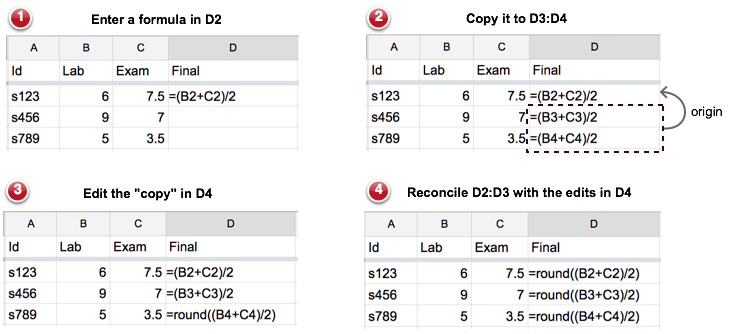
\includegraphics{images/grades.png}
\caption{\emph{Maintaining consistency among clones of formulas through
copy-paste tracking}}
\end{figure}

Figure 1 shows an example user interaction with a spreadsheet containing
student grades. In the first step the sheet contains just the Lab and
Exam grades of three students, and a formula for computing the average
of the two grades in D2. In the second step, the formula in cell D2 is
copied to D3 and D4. D3 and D4 are clones of D2, and this relation is
maintained by the system as an origin relation (visualized using the
arrow). In the third step, the clone in D4 is modified to apply rounding
to the computed average. Unlike in normal spreadsheets, however, this is
not the end of the story and XanaSheet will reconcile the original
formula of D2 and the other clone in D3 with the changes in D4.

A way to understand what is happening here, is to see spreadsheet
formulas as materialized or unfolded abstractions. The abstraction in
Fig. 1 is function \texttt{average(x,y)} for computing the average of
two grades. In ordinary programming such a function could, for instance,
be mapped over a list of pairs of grades to obtain a list of averages,
like \texttt{map(average,\ zip(Lab,\ Exam))}. In the spreadsheet of Fig.
1, however, the abstraction \texttt{average} does not really exist, but
is represented collectively by the set of all its inlined applications,
e.g.
\texttt{{[}(Lab{[}0{]}+Exam{[}0{]})/\ 2,\ (Lab{[}1{]}+Exam{[}1{]})/2,\ (Lab{[}2{]}+Exam{[}2{]})/2{]}}.
In a sense, each application is a clone of the same implicit prototype,
with parameters filled in with concrete data references. The tracking
relation induced by copy-paste actions, identifies which clones belong
to the same equivalence class. Therefore, editing one clone triggers
updating the clones which belong to the same class.

In some cases it might actually not be desired to maintain the origin
links between source and destination of copy-paste actions. XanaSheet
supports these situations by providing a special ``Paste and Detach''
action which severs the copy from its original (similar to ``Past and
Match Style'' common in many text editing systems). The example also
assumes that when a user edits a formula she always intends to edit the
whole class of clones. However, the system allows the user to edit only
this copy, or all copies at once (similar to changing ``Recurring
events'' in calendar applications).

\section{Semantics of Copy-Paste
Tracking}\label{semantics-of-copy-paste-tracking}

The previous section introduced copy-paste tracking from the perspective
of the user. In this section we describe our considerations regarding
the implementation. We have implemented an executable semantics of
copy-paste tracking for simulating interactive editing sessions with a
spreadsheet. The code can be found online here:
\url{https://github.com/Felienne/LiveSpreadsheets/tree/master/XanaSheet}.
We are currently working on an interactive prototype of XanaSheet.

A spreadsheet is a rectangular grid of cells where each cell is
identified by its \emph{address}, which are pairs \(An\) consisting of a
column letter \(A\) and a row index \(n\). User actions always operate
on one of more of these addresses. The origin relation between cells is
then modeled as a binary relation between such addresses. For instance,
the relation \(Org = \{\langle D3, D2\rangle,\langle D4, D2\rangle\}\)
captures the origin relation visualized in Figure 1 (2). In this case,
the relation states that the formulas in cell \(D3\) and cell \(D4\) are
copied from cell \(D2\).

Without loss of generality we assume users only use relative cell
referencing in formulas. That is, a cell reference consists of relative
row and column offsets starting from the current cell {[}@Sestoft{]}.
For instance, the reference to \texttt{B2} in Fig. 1 (1) is a relative
cell reference, is represented as \texttt{C-2R0} (``two columns left,
same row''). Relative cell referencing allows formulas to be moved
around across the grid without having to adjust explicit column names or
row indices.

Interacting with the spreadsheet not only updates the sheet itself, but
also maintains the origin relation. We describe the effect of the most
relevant edit operations on a cell \(c\):

\begin{itemize}
\item
  \emph{Entering a formula}: If \(c\) does not participate in any origin
  relation, it is is simply updated with the new formula, and the origin
  relation is updated with \(\langle c, c\rangle\) to model the fact
  that a new formula is its own origin. As a result, the origin relation
  is always reflexively closed. Otherwise, \(c\) has an origin, say
  \(c'\), and the cells that need to be updated are
  \(\{ c'' \;|\; \langle c'', c'\rangle \in Org \}\). By definition,
  this includes cell \(c\), and, by reflexivity of \(Org\), the source
  cell \(c'\) as well. .
\item
  \emph{Copying cell \(c\) to \(c'\)}: The contents of \(c\) is copied
  to \(c'\). If the contents is a formula, the origin relation needs to
  be updated as well. First, if \(c'\) has an existing origin, the
  corresponding pair is removed from the relation. Then the relation is
  extended based on the current copy operation: if \(c\) has an origin
  \(c''\), add \(\langle c', c''\rangle\), else add
  \(\langle c', c\rangle\). The check for the origin of \(c\) ensures
  that the origin relation is always transitively closed.
\item
  \emph{Inserting/removing a row or column}: after updating the sheet,
  the origin relation is adjusted so that cell addresses refer to their
  new locations. For instance, when inserting a row at position \(i\),
  the row components of all the cell addresses on rows \(\geq i\) in the
  origin relation needs to be shifted one down. In the case of removal,
  all pairs in the origin relation that contain coordinates on the
  removed row or column are removed.
\item
  \emph{Entering data}: cell \(c\) is updated with the new data. All
  pairs containing \(c\), either as source or target, are removed from
  the origin relation.
\end{itemize}

Note that copying a cell \(c\) to \(c'\) removes the origin entries of
\(c'\) (if any). An alternative design could interpret copying a formula
as a modification of the destination cell, and thus update all cells in
the class of \(c'\). In that case all such cells would get \(c\) as
their new origin.

Although in this section we have just discussed copy-paste tracking for
formulas, the same model can be applied equally well to copy-pasting of
data. In that case, the origin relation helps against inadvertently
duplicating input data. An interesting special case is the ``paste as
value'' operation. Instead of copying a formula, this operation copies
the computed value, thus completely disconnecting the destination cell
from its source. Tracking such copy-paste actions would probably not be
very useful: editing the pasted value would incur computing the inverse
of the original formula, and updating the input data accordingly!

\section{Related Work}\label{related-work}

Copy-paste tracking is a simple technique that is inspired by similar
concepts in domains as diverse as term rewriting, hypertext, clone
detection, prototypical inheritance , and view maintenance. Below we
briefly summarize representative related work in those areas.

\emph{Origin tracking}: Copy-paste tracking is directly inspired by
\emph{origin tracking} {[}@VanDeursenKT93{]}. In general, origin
tracking tries establish a relation between the input and output of some
computational process, such as a compiler, or program transformation.
Origin tracking, however, has numerous other applications in
visualization, debugging, and traceability. An application most similar
to our work is presented in {[}@InostrozaVdSE{]}, where origin tracking
is used to implement editable regions on generated code.

\emph{Transclusion}: Ted Nelson's concept of \emph{transclusion}
{[}@Nelson65{]} is a form of ``reference by inclusion'' where
transcluded data is presented through a ``live'' view: whenever the
transcluded content is updated, the views are updated as well. Our
origin relation provides a similar hyper-linking between cells. But
unlike in the case of transclusion, the relation is bidirectional:
changes to the original are propagated forward, but changes to copies
(references) are also propagated backwards (and then forwards again). A
similar concept is used in Subtext, where copying is the primary
mechanism for abstraction {[}@Subtext{]}.

\emph{Clone tracking} in software: Godfrey and Tu {[}@Godf2002{]}
proposed a method called \emph{origin analysis} which is a related to
both clone detection and the above described origin tracking, but aims
at deciding if a program entity was newly introduced or whether it if it
should more accurately be viewed as a renamed, moved, or otherwise
changed version of an previously existing entity. This laid the ground
for a tool called \emph{CloneTracker} that ``can automatically track
clones as the code evolves, notify developers of modifications to clone
regions, and support simultaneous editing of clone regions.''
{[}@Dual2007{]}.

\emph{Prototype-based inheritance}: Lieberman introduced prototypes to
implement shared behavior in object-oriented programming
{[}@LiebermanProto{]}. In prototype-based languages, objects are created
by cloning and existing object. The cloned object then inherits features
(methods, slots) from its prototype. The parent relation between objects
is similar to our origin relation. However, we are not aware of any
related work using this relation to propagate changes to clones back to
their parents.

\emph{Bidirectional transformation}: one way to look at copy-paste
tracking is to see copies as views on the original formula similar to
views in database systems. In particular, the copies are
\emph{updateable} views {[}@bancilhon1981update{]}. Different
manifestations of the view update problem have received considerable
attention recently in the context of \emph{lenses} {[}@Lenses{]} and
bidirectional transformation {[}@BX{]}. In the context of user
interfaces these concepts were pioneered by Meertens under the header of
``constraint maintenance'' {[}@Meertens{]}. In a certain sense,
copy-paste tracking supports a very basic class of constraint
maintenance where clones are simply synchronized to be equal.

\section{Conclusion}\label{conclusion}

Spreadsheet systems are the most popular live programming environments.
They adhere to the powerful direct manipulation style of simultaneously
editing data and code. Nevertheless, spreadsheets are known to be
extremely fault-prone, mainly because users have to use copy-paste
instead of user defined abstractions. Existing research has tried to
improve spreadsheets by introducing abstractions such as meta models or
user defined functions, but this compromises the direct manipulation
aspect that makes spreadsheets so attractive in the first place.

In this paper we propose XanaSheet: copy-paste tracking as way to both
have our cake and eat it too. Instead of introducing another level of
indirection, copy-paste tracking supports editing classes of formulas
originating at the same source, all at once. As a result, we get the
benefits of abstraction (reuse, sharing, ``single-point-of-change''),
without the incurring the burden of cognitive distance.

\emph{Outlook} Duplication of knowledge is ubiquitous is computing.
Copy-paste tracking can generalized to a broader scope by seeing it as
an example of abstractions that are presented to the user in a
materialized, expanded, unrolled, referenced, or instantiated state. The
relation between such views and the original is often many-to-one and
the views are often read only. Copy-paste tracking could provide a model
to make such user views of abstractions editable. Thus, copy-paste
tracking in its most general form supports direct manipulation in
interactive systems and allows users to maintain abstractions through
their multiple concretizations. We conclude by providing a tentative
list of examples where similar ideas could be applied:

\begin{longtable}[c]{@{}ll@{}}
\toprule
``Copy'' (many) & ``Source'' (one)\tabularnewline
\midrule
\endhead
Reference & Declaration\tabularnewline
Stack frame & Procedure call\tabularnewline
Inlining & Procedure\tabularnewline
Text output & Template\tabularnewline
Object & Class\tabularnewline
Styled element & Style sheet\tabularnewline
Denormalized view & Normalized database\tabularnewline
Unrolling & Loop\tabularnewline
\bottomrule
\end{longtable}

\section{References}\label{references}

\end{document}
